\vspace{-2mm}
\section{Letter}
\label{sxn:body}
\vspace{-1mm}

Recent work by Martin and Mahoney~\cite{MM18_TR} provides a Universal empirical metric that characterizes the amount of \emph{Implicit Self-Regularization} and, accordingly, 
the generalization capacity, for a wide range of widely available, best-in-class, pre-trained Deep Neural Networks (DNNs), such as AlexNet, VGG, ResNet, etc.   

Instead of looking worst-case bounds, they study the Empirical Spectral Density (ESD), $\rho(\lambda)$, of individual layer weight matrices, $\mathbf{W}$ (and convolutional feature maps), 
through the lens of Random Matrix Theory (RMT).  Looking in detail at a series of models, one observes that the individual layer ESDs  almost always follow a power law (PL) distribution

\begin{equation}
\rho(\lambda)\sim\lambda^{-\alpha}  ,
\label{eqn:eigenval_pl}
\end{equation}

where $\rho(\lambda)$ is the density of the eigenvalues $\lambda$ of the normalized layer correlation matrix 

\begin{equation}
 \mathbf{X} = \frac{1}{N}\mathbf{W}^{T}\mathbf{W}.
\end{equation}

The power law exponents nearly all lie within a universal range $\alpha\in[2,5]$,  in nearly every pre-trained architecture studied, e.g., across nearly $10,000$ layer
 weight matrices (and 2D feature maps), including DNNs pre-trained for computer vision tasks on ImageNet, and for several different NLP tasks.

\begin{figure}[H]
   \centering
   \subfigure[All power law exponents $\alpha$]{
     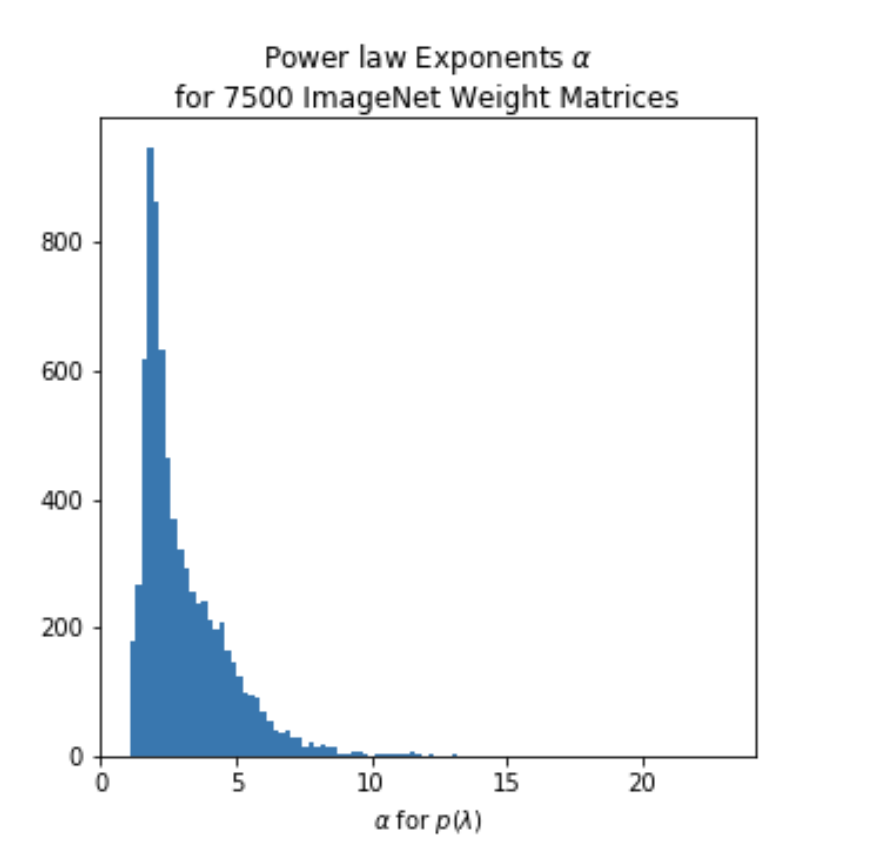
\includegraphics[scale=0.24]{img/power-law-histogram.png} 
     \label{fig:power-law-histogram}
   }
   \subfigure[ Average ${\alpha}$ vs Top5 error]{
      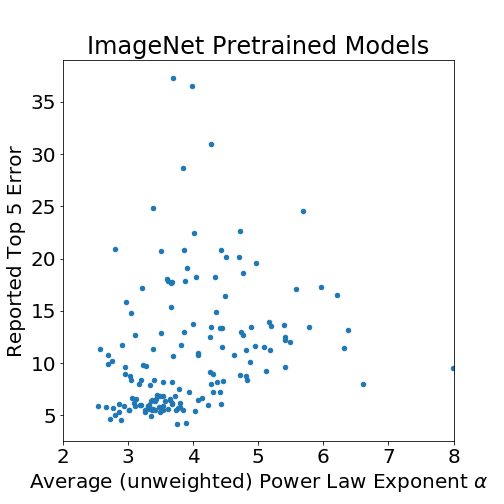
\includegraphics[scale=0.20]{img/Top5AvgAlpha.png}
      \label{fig:alphaTop5}
   }
   \caption{%
    Caption
   }
   \label{fig:alphas}
\end{figure}


Moreover, smaller $\alpha$ is correlated with better generalization accuracies, with $\alpha$ approaching a \emph{universal value}, $\alpha\rightarrow 2$,  at the lower limit of the
Fat Tailed RMT Universality class~\cite{MM18_TR} .  

In Statistical Physics, Universality of PL exponents is very special, and it suggests the presence of a deeper, underlying, \emph{Universal mechanism} driving the system dynamics~\cite{SornetteBook,BouchaudPotters03}.
It is this \emph{Heavy Tailed Mechanistic Universality} (HT-MU), as well call it, that originally motivated our study.  
HT-MU applies to the analysis of complicated systems, including many physical systems, traditional NNs~\cite{EB01_BOOK,nishimori01}, and even models of the dynamics of actual spiking neurons.
Indeed, the dynamics of learning in DNNs , and perhaps real neurons as well, 
seems to resemble a system near a phase transition, such as the phase boundary of spin glass, or a system displaying Self Organized Criticality (SOC), or a Jamming transition~\cite{GSdx18_TR,SGd18_TR}. 
Of course, we can not say which mechanism, if any, is at play. 
Instead, we use the machinery of  HT-RMT as a stand-in for a generative model of the weight matrices in DNNs, to catalog and model the HT behavior of DNNs.%

Based on these ideas, we develop a Universal capacity control metric $\hat{\alpha}$,  a weighted average of the layer power law (PL) exponents.
$(\alpha)$ of the DNN layer weight matrices:
\begin{equation}
\hat{\alpha}=\sum_{l\in L}\alpha_{l}\log\lambda_{l}^{max}  .
\end{equation}

where $\lambda_{l}^{max}$ is the  maximum eigenvalue  (i.e. Spectral norm) of layer correlation matrices $mathbf{W}_{l}$: 

\paragraph{Theory:} Our approach and intent differ from other theoretical studies, although we can related our results back to known results.
For example, Liao et al.~\cite{LMBx18_TR} used an appropriately-scaled, data-dependent Product Norm capacity control metric to bound the worst-case generalization 
error for several small (non production-quality, but still interesting) DNN models, and they showed that the bounds are remarkably tight.
There is, in fact, a large body of work on norm-based capacity control metrics, both recent, e.g.,~\cite{LMBx18_TR, SHNx17_TR,PLMx18_TR} and~\cite{NTS14_TR,NTS15,NBMS17_TR,BFT17_TR,YM17_TR,KKB17_TR,NBS17_TR,AGNZ18_TR,ACH18_TR,ZF18_TR}, as well as much older ~\cite{Bar97,MN09_TR}. 
These studies seek \emph{worst-case} complexity bounds, motivated to reconcile discrepancies with more traditional statistical learning theory, and they apply it to quite small NNs.
We seek an \emph{average-case} or \emph{typical case} (for realistic problems) complexity metric, viable in production to guide the development of better DNNs at scale.

Let us write the Energy Landscape (or optimization function) for a typical DNN with $L$ layers, with activation functions $h_{l}(\cdot)$, and with weight matrices and 
biases $\mathbf{W}_{l}$ and $\mathbf{b}_{l}$, as follows:
\begin{equation}
E=h_{L}(\mathbf{W}_{L}\times h_{L-1}(\mathbf{W}_{L-1}\times(\cdots)+\mathbf{b}_{L-1})+\mathbf{b}_{L})  .
\label{eqn:dnn_energy}
\end{equation}

Typically, this model would be trained on some labeled data $\{d_{i},y_{i}\}\in\mathcal{D}$, using Backprop\cite{BackProp}, by minimizing the loss $\mathcal{L}=\sum_{i\in\mathcal{D}}[E(d_{i})-y_{i}]$.

For simplicity, we do not indicate the structural details of the layers (e.g., Dense or not, Convolutions or not, Residual/Skip Connections, etc.) , nor
do we consider the details of the optimizer or the training process.

Each layer is defined by one or more layer 2D weight matrices $\mathbf{W}_{l}$, and/or the 2D feature maps $\mathbf{W}_{l,i}$ extracted directly from 2D Convolutional (Conv2D) layers.
(We have not yet analyzed LSTM or other complex Layers.)   A typical modern DNN may have anywhere between 5 and 5000 2D layer matrices / feature maps.

We can relate our universality metric to the more traditional, data dependent, VC-like product norm capacity metrics $\mathcal{C}$.
Define the \emph{worst-case} bound $\mathcal{C}$ as
\begin{equation}
\mathcal{C}\sim\Vert\mathbf{W}_{1}\Vert\times\Vert\mathbf{W}_{2}\Vert\cdots\Vert\mathbf{W}_{L}\Vert
\end{equation}
Using a standard trick from field theory, we consider the log product norm, which takes the form of an average log norm
\begin{eqnarray*}
\log\mathcal{C} &\sim& \log\bigg[\Vert\mathbf{W}_{1}\Vert\times\Vert\mathbf{W}_{2}\Vert\cdots\Vert\mathbf{W}_{L}\Vert\bigg]  \\
                &\sim& \bigg[\log\Vert\mathbf{W}_{1}\Vert+\log\Vert\mathbf{W}_{2}\Vert\cdots\log\Vert\mathbf{W}_{L}\Vert\bigg]  \\
                &\sim&  \langle\log\Vert\mathbf{W}\Vert\rangle=\dfrac{1}{N_{L}}\sum_{l}\log\Vert\mathbf{W}_{l}\Vert
\end{eqnarray*}

When $\Vert\mathbf{W}\Vert$ is the Spectral norm $\Vert\mathbf{W}\Vert_{2}\sim\lambda_{max}$, then $\hat{\alpha}$ is a weighted average of the log 
 product Spectral norm, where the weights are power law exponents $\alpha$. In this sense, our universal metric $\hat{\alpha}$ behaves
 like an \emph{average-case} version of what is a worst-case bound, and is more suitable for applying to large, production DNNs.
 
When $\Vert\mathbf{W}\Vert$ is the Frobenius norm $\Vert\mathbf{W}\Vert^{2}_{F}$, we can use results of Heavy Tailed RMT to interpret the PL
exponents $\alpha$ as a type of Soft Rank.  Specifically,, when $\alpha$ is very small, we can relate $\alpha$ to the more familiar
 Stable Rank $\mathcal{R}^{log}_{s}$, expressed in log-units (and up to the $\frac{1}{N}$ scaling):
 \begin{equation}
 \mathcal{R}^{log}_{s}:=\dfrac{\log\Vert\mathbf{W}\Vert^{2}_{F}}{\log\lambda^{max}}  \approx \alpha  .
\end{equation}
Using this, one could implement our capacity metric as a regularizer to improve DNN training by
implementing a Stable Rank regularizer (similar to how Spectral norm regularization is implemented).


\paragraph{Methodology:} To evaluate our metric, we introduce a new methodology to analyze the performance of large-scale pre-trained DNNs, 
 including the VGG and ResNet series of models, as well nearly 200 other widely available models, and study how the capacity metrics correlate with the reported test accuracies.
 
 This offers several advantages, most notably
 \begin{itemize}
 \item we do not need access to the ImageNet data, just the pretrained models (i.e as distributed with PyTorch, on github, and/or from the ModelZoo), and
 \item our results are easily reproducible.      To make things more reproducible, we provide a python command tool, weightwatcher~\cite{weightwatcher_pagkage}, 
  that works with both  PyTorch (v1) and Keras (v2) models and computes a wide range of average log capacity metrics.
 \end{itemize}
 
We apply our Universal capacity control metric $\hat{\alpha}$ to a wide range of large-scale pre-trained production-level DNNs,
Notice, for Linear DNN layers, we can simply replace the log Norm with our metric, whereas for Conv2D Layers, we associate 
the ``Norm'' of the 4-index Tensor $\mathbf{W}_{l}$ to the sum of the $n_{l}=c\times d$ terms for each feature map.

\begin{eqnarray*}
\text{Linear Layer:} & & \log\Vert\mathbf{W}_{l}\Vert
%\quad 
\rightarrow 
%\quad 
\alpha_{l}\log\lambda_{l}^{max}  \\
\text{Conv2D Layer:} & & \log\Vert\mathbf{W}_{l}\Vert
%\quad 
\rightarrow 
%\quad 
\sum_{i=1}^{n_{l}}\alpha_{l,i} \log\lambda_{l,i}^{max} , 
\end{eqnarray*}

\paragraph{Results:} 
Our Universal metric correlates very well with the reported average test accuracies across many series of pre-trained DNNs.

\begin{figure}[H]
   \centering
   \subfigure[$\hat{\alpha}$ for VGG series]{
      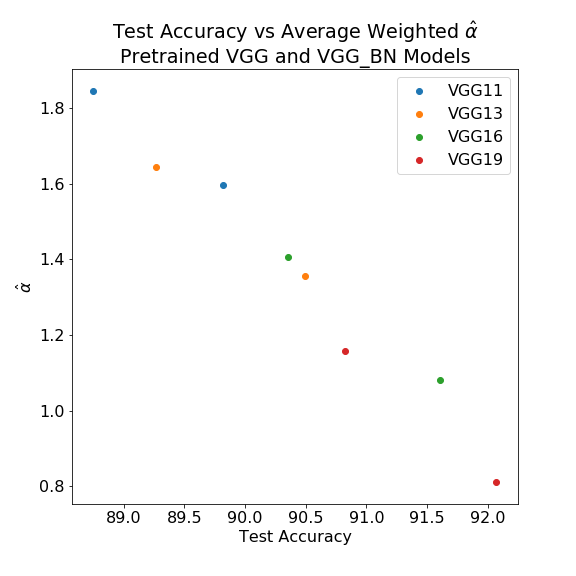
\includegraphics[scale=0.13]{img/vgg-w_alphas.png}
      \label{fig:vgg_alphahat}
   }
   \subfigure[$\hat{\alpha}$ for ResNet series]{
      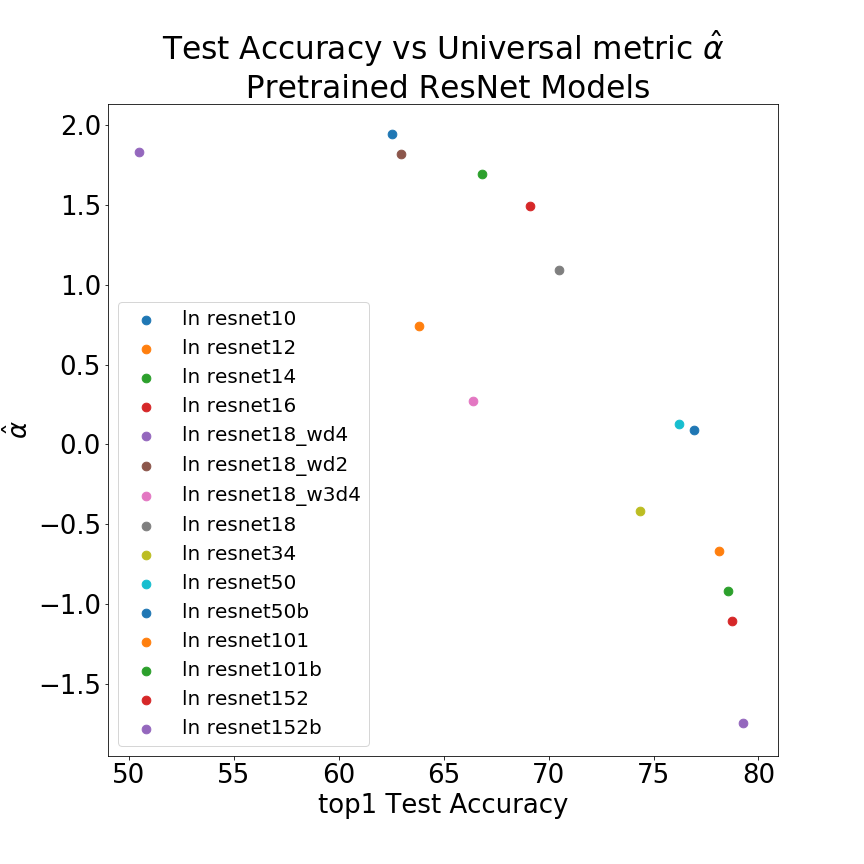
\includegraphics[scale=0.11]{img/ResNet-w_alphas.png}
      \label{fig:resnet_alphahat}
   }
   \caption{
      Top 1 Test Accuracy versus the
      Universal, weighted average PL exponent $\hat{\alpha}$
      for pre-trained VGG and    ResNet Architectures and DNNs.  
           }
   \label{fig:bothmodels}
\end{figure}

DISCUSS FIGURE IN DETAIL, CAN ADD 1 more BELOW and discuss



\begin{figure}[H]
   \centering
    \subfigure[  $\hat{\alpha}$ vs Top1 error]{
      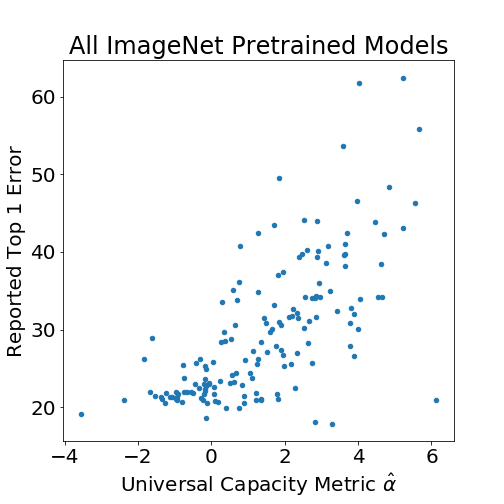
\includegraphics[scale=0.20]{img/Top1AlphaHat.png}
      \label{fig:alphahatTop1}
   }
   \caption{%
    Caption: we have room for 1 more 
   }
   \label{fig:alphahats}
\end{figure}


Our empirical results are, to our knowledge, the first time such theoretical capacity 
metrics have been reported to predict (trends in) the test accuracy for \emph{pre-trained production-level} DNNs.
In particular, this illustrates the usefulness of these norm-based metrics beyond smaller models such as MNIST, CIFAR10, and CIFAR100. 
Our  results can be reproduced with the \texttt{WeightWatcher} package%
%~\cite{weightwatcher_pagkage}; 
\footnote{\url{https://pypi.org/project/WeightWatcher/}};
and our
results suggest that our ``practical theory'' approach is fruitful more generally for engineering good algorithms for realistic large-scale DNNs.

\paragraph{Comparison with other metrics}

\paragraph{Discussion}

We have presented an \emph{unsupervised} capacity control metric which predicts trends in test accuracies of a trained DNN---without peeking at the test data. 
This complexity metic, $\hat{\alpha}$ of Eqn.~(\ref{eqn:alpha_hat_specific}), is a weighted average of the PL exponents $\alpha$ for each layer weight matrix, where $\alpha$ is defined in the recent HT-SR Theory~\cite{MM18_TR}, and where the weights are the largest eigenvalue $\lambda^{max}$ of the correlation matrix $\mathbf{X}$.  
%
We examine several commonly-available, pre-trained, production-quality DNNs by plotting $\hat{\alpha}$ versus the reported test accuracies.
This covers classes of DNN architectures including the VGG models, ResNet, DenseNet, etc. 
In nearly every class, and except for a few counterexamples, smaller $\hat{\alpha}$ corresponds to better average test accuracies, thereby providing a strong predictor of model quality.

 It is worth emphasizing that 
we are taking a very non-standard approach (at least for the DNN and ML communities).
We did not train/retrain lots and lots of (typically rather small) models, analyzing training/test curves, trying to glean from them bits of insight that might then extrapolate to more realistic models.
Instead, we take advantage of the fact that there already exist many (typically rather large) publicly-available pre-trained models, and we analyze the properties of these models.
That is, we viewed these publicly-available pre-trained models as artifacts of the world that achieve state-of-the-art performance in computer vision, NLP, and related applications; and we attempted to understand why.
and we then extracted data-dependent metrics to predict their generalization performance on production-quality models.
Given well-known challenges associated with training, and given our results here as well as other recent results~\cite{MM18_TR},
we suggest that this methodology be applied more generally.

In the context of theoretical physics...discuss spin glass models and LeCuns approach to complexity


